\begin{figure}[h!]
	\centering
	
	
	
	\tikzset{every picture/.style={line width=0.75pt}} %set default line width to 0.75pt        
	
	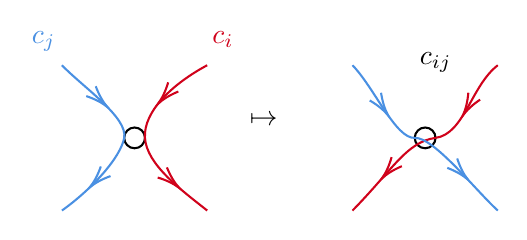
\begin{tikzpicture}[x=0.75pt,y=0.75pt,yscale=-1,xscale=1]
		%uncomment if require: \path (0,300); %set diagram left start at 0, and has height of 300
		
		%Shape: Circle [id:dp20341541956461162] 
		\draw   (140,65) .. controls (140,62.24) and (142.24,60) .. (145,60) .. controls (147.76,60) and (150,62.24) .. (150,65) .. controls (150,67.76) and (147.76,70) .. (145,70) .. controls (142.24,70) and (140,67.76) .. (140,65) -- cycle ;
		%Curve Lines [id:da2859009285050971] 
		\draw [color={rgb, 255:red, 208; green, 2; blue, 27 }  ,draw opacity=1 ]   (180,30) .. controls (163.5,38.84) and (149.17,52.17) .. (150,65) .. controls (150.83,77.83) and (167.17,89.84) .. (180,100) ;
		\draw [shift={(156.31,48.57)}, rotate = 312.09] [color={rgb, 255:red, 208; green, 2; blue, 27 }  ,draw opacity=1 ][line width=0.75]    (10.93,-3.29) .. controls (6.95,-1.4) and (3.31,-0.3) .. (0,0) .. controls (3.31,0.3) and (6.95,1.4) .. (10.93,3.29)   ;
		\draw [shift={(166.44,89.03)}, rotate = 222.39] [color={rgb, 255:red, 208; green, 2; blue, 27 }  ,draw opacity=1 ][line width=0.75]    (10.93,-3.29) .. controls (6.95,-1.4) and (3.31,-0.3) .. (0,0) .. controls (3.31,0.3) and (6.95,1.4) .. (10.93,3.29)   ;
		%Curve Lines [id:da8106417469658391] 
		\draw [color={rgb, 255:red, 74; green, 144; blue, 226 }  ,draw opacity=1 ]   (110,30) .. controls (120.5,40.84) and (141.84,55.17) .. (140,65) .. controls (138.16,74.83) and (123.84,90.17) .. (110,100) ;
		\draw [shift={(131.86,50.09)}, rotate = 224.05] [color={rgb, 255:red, 74; green, 144; blue, 226 }  ,draw opacity=1 ][line width=0.75]    (10.93,-3.29) .. controls (6.95,-1.4) and (3.31,-0.3) .. (0,0) .. controls (3.31,0.3) and (6.95,1.4) .. (10.93,3.29)   ;
		\draw [shift={(123.39,88.86)}, rotate = 314.65] [color={rgb, 255:red, 74; green, 144; blue, 226 }  ,draw opacity=1 ][line width=0.75]    (10.93,-3.29) .. controls (6.95,-1.4) and (3.31,-0.3) .. (0,0) .. controls (3.31,0.3) and (6.95,1.4) .. (10.93,3.29)   ;
		%Shape: Circle [id:dp752571342246523] 
		\draw   (280,65) .. controls (280,62.24) and (282.24,60) .. (285,60) .. controls (287.76,60) and (290,62.24) .. (290,65) .. controls (290,67.76) and (287.76,70) .. (285,70) .. controls (282.24,70) and (280,67.76) .. (280,65) -- cycle ;
		%Curve Lines [id:da8927632362609036] 
		\draw [color={rgb, 255:red, 208; green, 2; blue, 27 }  ,draw opacity=1 ]   (320,30) .. controls (307.17,39.84) and (303.84,63.17) .. (290,65) .. controls (276.16,66.83) and (269.17,80.5) .. (250,100) ;
		\draw [shift={(303.1,54.32)}, rotate = 300.5] [color={rgb, 255:red, 208; green, 2; blue, 27 }  ,draw opacity=1 ][line width=0.75]    (10.93,-3.29) .. controls (6.95,-1.4) and (3.31,-0.3) .. (0,0) .. controls (3.31,0.3) and (6.95,1.4) .. (10.93,3.29)   ;
		\draw [shift={(264.07,84.65)}, rotate = 311.47] [color={rgb, 255:red, 208; green, 2; blue, 27 }  ,draw opacity=1 ][line width=0.75]    (10.93,-3.29) .. controls (6.95,-1.4) and (3.31,-0.3) .. (0,0) .. controls (3.31,0.3) and (6.95,1.4) .. (10.93,3.29)   ;
		%Curve Lines [id:da30399005579052596] 
		\draw [color={rgb, 255:red, 74; green, 144; blue, 226 }  ,draw opacity=1 ]   (250,30) .. controls (260.5,40.84) and (270.84,65.5) .. (280,65) .. controls (289.16,64.5) and (309.5,90.5) .. (320,100) ;
		\draw [shift={(267.16,54.16)}, rotate = 235.87] [color={rgb, 255:red, 74; green, 144; blue, 226 }  ,draw opacity=1 ][line width=0.75]    (10.93,-3.29) .. controls (6.95,-1.4) and (3.31,-0.3) .. (0,0) .. controls (3.31,0.3) and (6.95,1.4) .. (10.93,3.29)   ;
		\draw [shift={(305.59,85.09)}, rotate = 226.4] [color={rgb, 255:red, 74; green, 144; blue, 226 }  ,draw opacity=1 ][line width=0.75]    (10.93,-3.29) .. controls (6.95,-1.4) and (3.31,-0.3) .. (0,0) .. controls (3.31,0.3) and (6.95,1.4) .. (10.93,3.29)   ;
		
		% Text Node
		\draw (199,52.4) node [anchor=north west][inner sep=0.75pt]    {$\mapsto $};
		% Text Node
		\draw (181,12.4) node [anchor=north west][inner sep=0.75pt]  [color={rgb, 255:red, 208; green, 2; blue, 27 }  ,opacity=1 ]  {$c_{i}$};
		% Text Node
		\draw (94,12.4) node [anchor=north west][inner sep=0.75pt]  [color={rgb, 255:red, 74; green, 144; blue, 226 }  ,opacity=1 ]  {$c_{j}$};
		% Text Node
		\draw (281,22.4) node [anchor=north west][inner sep=0.75pt]  [color={rgb, 255:red, 0; green, 0; blue, 0 }  ,opacity=1 ]  {$c_{ij}$};
		
		
	\end{tikzpicture}
\end{figure}